\documentclass{exam}

\usepackage{siunitx} 
\usepackage{graphicx}
\usepackage[fleqn]{amsmath}
\usepackage{cancel}
\usepackage{float}
\usepackage{mdwlist}
\usepackage{booktabs}
\usepackage{cancel}
\usepackage{polynom}
\usepackage{caption}
\usepackage{fullpage}
\usepackage{comment}

\newcommand{\degree}{\ensuremath{^\circ}} 
\everymath{\displaystyle}

% \begin{figure}[H]
%   \centering
%   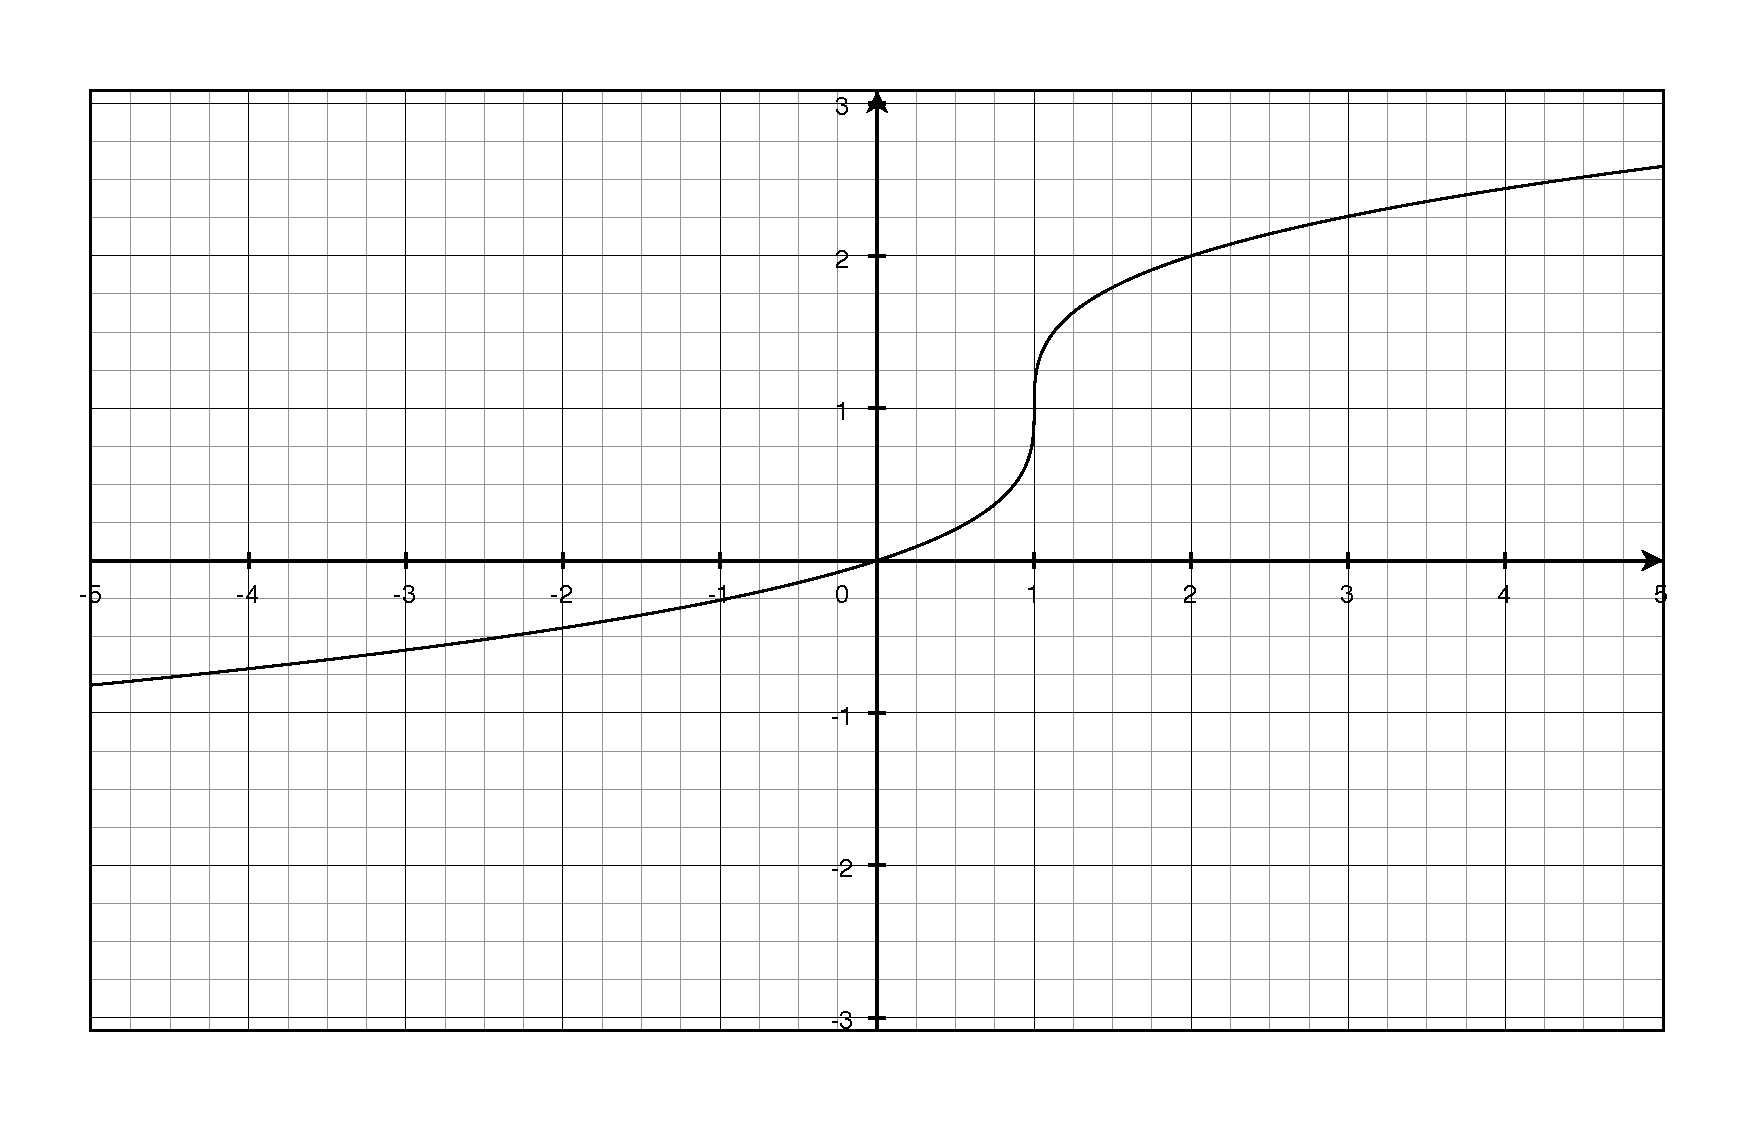
\includegraphics[scale=.3]{question7.eps}
%   \caption*{question 7}
% \end{figure}

% \begin{tabular}{cc}
%   \toprule
%   period & amplitude \\
%   \midrule
%     $\pi$ & $2$ \\
%   \bottomrule
% \end{tabular}

\printanswers
\excludecomment{comment}

\ifprintanswers 
  \usepackage{2in1, lscape} 
\fi

\author{}
\date{\today}
\title{Math 142 \\ Homework One}

\begin{document}

  \maketitle

  \section{Homework}

  Section 5.1: 

  \section{Extra Credit}

  TO DO

  \ifprintanswers
    \begin{solution}
      TO DO
    \end{solution}

    \pagebreak

    \section{Section 5.1}
    \begin{description}

      \item[7]
        \begin{align*}
          \left( \frac{3}{5} \right)^2 + y^2 & = 1 \\
          y                                  & = \pm \frac{4}{5} \\
        \end{align*}

        The point in quadrant III is: $\boxed{ \left( -\frac{3}{5}, -\frac{4}{5} \right) }$.

      \item[8]
        \begin{align*}
          x^2 + \left( - \frac{7}{25} \right)^2 & = 1 \\
          x                                     & = \pm \frac{3 \sqrt{2}}{5} \\
        \end{align*}

        The point in quadrant IV is: $\boxed{ \left( \frac{3 \sqrt{2}}{5}, -\frac{7}{25} \right) }$.

      \item[9]
        \begin{align*}
          x^2 + \left( \frac{1}{3} \right)^2 & = 1 \\
          x                                  & = \pm \frac{2 \sqrt{2}}{3} \\
        \end{align*}

        The point in quadrant IV is: $\boxed{ \left( - \frac{2 \sqrt{2}}{3}, \frac{1}{3} \right) }$.

      \item[10]
        \begin{align*}
          \left( \frac{2}{5} \right)^2 + y^2 & = 1 \\
          y                                  & = \pm \frac{\sqrt{21}}{5} \\
        \end{align*}

        The point in quadrant IV is: $\boxed{ \left( \frac{2}{5}, \frac{\sqrt{21}}{5} \right) }$.

      \item[15]
        \begin{align*}
          x^2 + \left( \frac{2}{3} \right)^2 & = 1 \\
          x                                  & = \pm \frac{\sqrt{5}}{3} \\
        \end{align*}

        The point is: $\boxed{ \left( - \frac{\sqrt{5}}{3}, \frac{2}{3} \right) }$.

      \item[16]
        \begin{align*}
          x^2 + \left( - \frac{\sqrt{5}}{5} \right)^2 & = 1 \\
          x                                  & = \pm \frac{2 \sqrt{5}}{5} \\
        \end{align*}

        The point is: $\boxed{ \left( \frac{2 \sqrt{5}}{5}, \frac{\sqrt{5}}{5} \right) }$.

      \item[17]
        \begin{align*}
          \left( - \frac{\sqrt{2}}{3} \right)^2 + y^2 & = 1 \\
          y                                           & = \pm \frac{\sqrt{7}}{3} \\
        \end{align*}

        The point is: $\boxed{ \left( \frac{\sqrt{2}}{3}, - \frac{\sqrt{7}}{3} \right) }$.

      \item[18]
        \begin{align*}
          \left( - \frac{2}{5} \right)^2 + y^2 & = 1 \\
          y                                    & = \pm \frac{\sqrt{21}}{3} \\
        \end{align*}

        The point is: $\boxed{ \left( - \frac{2}{5}, \frac{\sqrt{21}}{3} \right) }$.

      \item[19]
        \begin{tabular}{cc}
          \toprule
          $t$ & terminal point \\
          \midrule
          $0$ & (1, 0) \\
          $\frac{\pi}{4}$ & $\left( \frac{\sqrt{2}}{2}, \frac{\sqrt{2}}{2} \right)$ \\

          $\frac{\pi}{2}$ & $\left( 0, 1 \right)$ \\
          $\frac{3 \pi}{4}$ & $\left( -\frac{\sqrt{2}}{2}, \frac{\sqrt{2}}{2} \right)$ \\

          $\pi$ & $\left( -1, 0 \right)$ \\
          $\frac{5 \pi}{4}$ & $\left( -\frac{\sqrt{2}}{2}, -\frac{\sqrt{2}}{2} \right)$ \\

          $\frac{3 \pi}{2}$ & $\left( 0, -1 \right)$ \\
          $\frac{7 \pi}{4}$ & $\left( \frac{\sqrt{2}}{2}, -\frac{\sqrt{2}}{2} \right)$ \\
          \bottomrule
        \end{tabular}

      \item[20]
        \begin{tabular}{cc}
          \toprule
          $t$ & terminal point \\
          \midrule
          $0$             & $(1, 0)$ \\
          $\frac{\pi}{6}$ & $\left( \frac{\sqrt{3}}{2}, \frac{1}{2} \right)$ \\
          $\frac{\pi}{3}$ & $\left( \frac{1}{2}, \frac{\sqrt{3}}{2} \right)$ \\

          \midrule
          $\frac{\pi}{2}$   & $(0, 1)$ \\
          $\frac{2 \pi}{3}$ & $\left( -\frac{1}{2}, \frac{\sqrt{3}}{2} \right)$ \\
          $\frac{5 \pi}{6}$ & $\left( -\frac{\sqrt{3}}{2}, \frac{1}{2} \right)$ \\

          \midrule
          $\pi$             & $(-1, 0)$ \\
          $\frac{7 \pi}{6}$ & $\left( -\frac{\sqrt{3}}{2}, -\frac{1}{2} \right)$ \\
          $\frac{4 \pi}{3}$ & $\left( -\frac{1}{2}, -\frac{\sqrt{3}}{2} \right)$ \\

          \midrule
          $\pi$              & $(0, -1)$ \\
          $\frac{5 \pi}{3}$  & $\left( \frac{1}{2}, -\frac{\sqrt{3}}{2} \right)$ \\
          $\frac{11 \pi}{6}$ & $\left( \frac{\sqrt{3}}{2}, -\frac{1}{2} \right)$ \\
          
          \bottomrule
        \end{tabular}

      \item[21] $t = \frac{\pi}{2}$; terminal point: $\boxed{ \left( 0, 1 \right) }$

      \item[22] $t = \frac{3 \pi}{2}$; terminal point: $\boxed{ \left( 0, -1 \right) }$

      \item[23] $t = \frac{5 \pi}{6}$; terminal point: $\boxed{ \left( - \frac{\sqrt{3}}{2}, \frac{1}{2} \right) }$

      \item[24] $t = \frac{7 \pi}{6}$; terminal point: $\boxed{ \left( - \frac{\sqrt{3}}{2}, - \frac{1}{2} \right) }$

      \item[25] $t = -\frac{\pi}{3}$; terminal point: $\boxed{ \left( \frac{1}{2}, - \frac{\sqrt{3}}{2}  \right) }$

      \item[26] $t = \frac{5 \pi}{3}$; terminal point: $\boxed{ \left( \frac{1}{2}, - \frac{\sqrt{3}}{2}  \right) }$

      \item[27] $t = \frac{2 \pi}{3}$; terminal point: $\boxed{ \left( - \frac{1}{2}, \frac{\sqrt{3}}{2}  \right) }$

      \item[28] $t = -\frac{\pi}{2}$; terminal point: $\boxed{ \left( 0, -1 \right) }$

      \item[29] $t = - \frac{3 \pi}{4}$; terminal point: $\boxed{ \left( - \frac{\sqrt{2}}{2}, - \frac{\sqrt{2}}{2}  \right) }$
        
      \item[30] $t = \frac{11 \pi}{6}$; terminal point: $\boxed{ \left( \frac{\sqrt{3}}{2}, - \frac{1}{2}  \right) }$

      \item[31]
        \begin{enumerate}[a]
          \item $\boxed{ \left( - \frac{3}{5}, \frac{4}{5} \right) }$
        
          \item $\boxed{ \left( \frac{3}{5}, - \frac{4}{5} \right) }$

          \item $\boxed{ \left( - \frac{3}{5}, - \frac{4}{5} \right) }$

          \item $\boxed{ \left( - \frac{3}{5}, - \frac{4}{5} \right) }$

        \end{enumerate}

      \item[32]
        \begin{enumerate}[a]
          \item $\boxed{ \left( \frac{3}{4}, - \frac{\sqrt{7}}{4} \right) }$
        
          \item $\boxed{ \left( \frac{3}{4}, \frac{\sqrt{7}}{4} \right) }$

          \item $\boxed{ \left( - \frac{3}{4}, \frac{\sqrt{7}}{4} \right) }$

          \item $\boxed{ \left( - \frac{3}{4}, - \frac{\sqrt{7}}{4} \right) }$

        \end{enumerate}

      \item[33] 
        \begin{enumerate}[a]
          \item $\frac{5 \pi}{4} - \pi   = \boxed{ \frac{\pi}{4} }$
          \item $\frac{7 \pi}{3} - 2 \pi = \boxed{ \frac{\pi}{3} }$
          \item $\frac{4 \pi}{3} - \pi   = \boxed{ \frac{\pi}{3} }$
          \item $\frac{\pi}{6} - 0       = \boxed{ \frac{\pi}{6} }$
        \end{enumerate}
        
      \item[34] 
        \begin{enumerate}[a]
          \item $ \pi - \frac{5 \pi}{6}   = \boxed{ \frac{\pi}{6} }$
          \item $\frac{7 \pi}{6} - \pi    = \boxed{ \frac{\pi}{6} }$
          \item $4 \pi - \frac{11 \pi}{3} = \boxed{ \frac{\pi}{3} }$
          \item $2 \pi - \frac{7 \pi}{4}  = \boxed{ \frac{\pi}{4} }$
        \end{enumerate}
        
      \item[35] 
        \begin{enumerate}[a]
          \item $\pi - \frac{5 \pi}{7} = \boxed{ \frac{2 \pi}{7} }$
          \item $\pi - \frac{7 \pi}{9} = \boxed{ \frac{2 \pi}{9} }$
          \item $\pi - 3         \approx \boxed{ 0.1416 }$
          \item $2 \pi - 5       \approx \boxed{ 1.2832 }$
        \end{enumerate}

      \item[36] 
        \begin{enumerate}[a]
          \item $\frac{11 \pi}{5} - 2 \pi = \boxed{ \frac{\pi}{11} }$
          \item $\frac{9 \pi}{7} - \pi    = \boxed{ \frac{2 \pi}{7} }$
          \item 2 \pi - 6           \approx \boxed{ 0.2832 }$
        \end{enumerate}

    \end{description}
  \else
    \vspace{1 cm}
    \begin{quote}
      \begin{em}
        TO DO
      \end{em}
    \end{quote}
    \hspace{1 cm} --Henry David Thoreau
  \fi

\end{document}

